\documentclass[a4paper,12pt]{article}
\usepackage[utf8]{inputenc}
\usepackage[spanish, english]{babel}
\usepackage{amsmath}
\usepackage{graphicx}
\usepackage{hyperref}
\usepackage{geometry}
\usepackage{enumitem}
\geometry{margin=1in}

\begin{document}
\begin{titlepage}      
        \begin{center}
            
            {\LARGE Universidad Distrital Francisco José de Caldas\\[0.5cm]
			%{\color{blue} \rule{\textwidth}{1pt}}
			
			% -------------------------------
			% You need to edit some details here
			% -------------------------------  
            \linespread{1.2}\huge {
                %%%%%%%%%%%%%%%%%%%%%%%%%%%%
                %TODO: 1 TITLE of Your PROJECT 
                %%%%%%%%%%%%%%%%%%%%%%%%%%%%
                % change the following line                
                Systems Analysis: Toxic Comment Classification Challenge
            
            }}
            \linespread{1}~\\[5cm]
			%{\color{blue} \rule{\textwidth}{1pt}}
            {\Large 
                %%%%%%%%%%%%%%%%%%%%%%%%%%%%
                %TODO: 2 YOUR NAME
                %%%%%%%%%%%%%%%%%%%%%%%%%%%%             
                % change the following line
                Hugo Mojica Angarita  20232020034 \\ Laura Paez Cifuentes 20232020055\\ Andrey Camilo Gonzales Caceres 20231020070
                % change end             
            }\\[8cm] 
            

            {\large 
                %%%%%%%%%%%%%%%%%%%%%%%%%%%%
                %TODO: 3 YOUR NAME Supervisor's name(s)
                %%%%%%%%%%%%%%%%%%%%%%%%%%%%             
                % change the following line                
                \emph{Professor:} SIERRA VIRGUEZ CARLOS ANDRÉS}\\[1cm] % if applicable
            
    		% PLEASE DO NOT CHANGE THIS TEXT %
            \large System analysis and Design\\
            %%%
            %TODO:  verify your degree name
            \large Systems Engineering\\
            %% 
            \today
            \vfill
            % Please update this date you can use \date{April 2020} for fixed date
        \end{center}
    \end{titlepage}



\section*{Selected Competition: Toxic Comment Classification Challenge}

\textit{“The Conversation AI team, a research initiative founded by Jigsaw and Google (both a part of Alphabet), are working on tools to help improve online conversation. One area of focus is the study of negative online behaviors, like toxic comments (comments that are rude, disrespectful or otherwise likely to make someone leave a discussion). So far they’ve built a range of publicly available models served through the Perspective API, including toxicity. But the current models still make errors, and they don’t allow users to select which types of toxicity they’re interested in finding (e.g. some platforms may be fine with profanity, but not with other types of toxic content).
In this competition, you’re challenged to build a multi-headed model that’s capable of detecting different types of toxicity like threats, obscenity, insults, and identity-based hate better than Perspective’s current models. You’ll be using a dataset of comments from Wikipedia’s talk page edits. Improvements to the current model will hopefully help online discussion become more productive and respectful.”
”}

\section*{1. Key Elements of the Competition}
The data sets given in the competition are designed to train, test and analyze toxicity detection models.
\subsection*{Key Files}
\begin{itemize}
 \item The dataset includes many comments that have been classified by human evaluators for toxic behavior.
\item \textbf{Training set (\texttt{train.csv}):} It is a training set containing comments with their binary tags.
    \item \textbf{Test files:} This file contains unlabeled comments, the comments on which the models should predict toxicity. It is used to generate predictions that are then evaluated in the Kaggle Leaderboard.
\end{itemize}
\subsection*{Features}
\begin{itemize}
\item \textbf{Toxicity labels:} For example, \texttt{severe\_toxicity}, \texttt{obscene}, \texttt{identity\_attack}, etc. These variables help to understand the multidimensionality of toxicity: not all toxic comments are the same.
\item \textbf{Identity mentions:} Indicate whether the comment mentions features such as male, female, black, \texttt{sexual\_orientation}, etc. This is essential to evaluate if the model is systematically penalizing certain groups by mentioning their identity without insulting them.
\item \textbf{Metadata:} Such as dates, identifiers, and annotator counters.
\end{itemize}
\subsection*{Target Variables}
\begin{itemize}
\item \textbf{toxicity\_annotator\_count:} Number of annotators who evaluated the toxicity.
\item \textbf{identity\_annotator\_count:} Number of annotators who identified identity mentions.
\item \textbf{target:} Main target variable as it indicates the fraction of annotators who considered a comment to be toxic. Its value is a number between 0 and 1, for example, if \texttt{target} = 0.75 means that 75\% of the annotators consider the comment toxic.
\end{itemize}
\subsection*{Additional Considerations}
\begin{itemize}
\item Kaggle provided special metrics to measure this behavior: Subgroup AUC, BPSN AUC (Background Positive, Subgroup Negative), BNSP AUC (Background Negative, Subgroup Positive).
\end{itemize}

\section*{2. Relationship Mapping}

\subsection*{2.1. System Elements and Their Relationships}
\begin{itemize}
\item \textbf{Input (comments: comment\_text):} Input element of string type. It contains the comments to be analyzed from the users, varying from neutral phrases to insults, threats, humor, and affirmations. It is important to consider comments that seem toxic but may be sarcastic, as well as the context of each one.
\item \textbf{Identity annotations:} Variables that indicate a mention. They have continuous values from 0.0 to 1.0, where the number represents the fraction of annotators who think that identity has been explicitly or implicitly mentioned.
\textbf{Examples of identity:}
\begin{itemize}
\item Gender: male, female, transgender, other\_gender
\item Race/ethnicity: black, white, latino, asian, other\_race\_or\_ethnicity
\item Religion: christian, muslim, jewish, buddhist, atheist, other\_religion
\item Sexual orientation: heterosexual, homosexual\_gay\_or\_lesbian, bisexual, other\_sexual\_orientation
\item Health conditions/disability: physical\_disability, psychiatric\_or\_mental\_illness
\end{itemize}
\item \textbf{Toxicity Tags:} In the dataset, the columns perceive different types of toxicity in a comment:
\begin{itemize}
\item \texttt{toxicity}: general level of toxicity.
\item \texttt{severe\_toxicity}: extreme toxicity and intense verbal violence.
\item \texttt{obscene}: vulgar or inappropriate language.
\item \texttt{identity\_attack}: attacks directed at identity groups.
\item \texttt{insult}: personal or collective insults.
\item \texttt{threat}: explicit or implicit threats.
\item \texttt{sexual\_explicit}: explicitly sexual content.
\end{itemize}
\item \textbf{Target Variable (target):} It is a variable between 0.0 and 1.0 that represents the level of toxicity that the annotators considered the comment to have. This variable is the one that the model must predict.
\end{itemize}

\subsection*{2.2. System Information Flow}
The flow of information in this context is useful to understand how information flows within the system, such as what data is generated, its destination, who uses it, and how it changes. This helps to visualize the relationships more clearly.
\begin{enumerate}
\item \textbf{Step 1: Text input.} The user's comment is received as input into the system.
\item \textbf{Step 2: Processing.} The input is cleaned, leaving only a string without symbols, capital letters, or extra punctuation. In addition to tokenizing it (processing the natural language to make it easier for machines to understand), using some model.
\item \textbf{Step 3: Identity mentions.} The identity mentions of the comment are analyzed, and sensitive mentions are identified. This can be achieved by using rules or an additional model.
\item \textbf{Step 4: Classification of the comment.} The model must process the comment and make a toxicity prediction to store it in the target variable. As an addition, predictions for \texttt{severe\_toxicity}, \texttt{identity\_attack}, etc., can be added.
\item \textbf{Step 5: System output.} Returns the toxicity probability, the target variable.
\end{enumerate}

\subsection*{2.3. System Constraints}
The competition provides certain rules, such as the use of public data or data provided by Kaggle. Regarding RAM, the code must run within a limited time. Additionally, the data provided cannot be modified.

It is important to emphasize some ethical rules, such as avoiding training the model to develop discrimination towards identity groups, as the model must minimize these behaviors.

\subsection*{2.4. System Boundaries}
Defining the boundaries helps us to identify what part of the system is and what is outside its control.

The elements that are within the system boundaries are: input data, text preparation process, classification model, evaluation metrics, model validation, and output.

The elements that are outside the boundaries of the system are: the moral or legal interpretation that is outside the perception contained in the data, the generation of real-time responses, and the perception of the language of all the different social identities.

In conclusion, the system helps us to mitigate toxicity in a moderation ecosystem; however, it does not fully address the social impact and ensure structured justice.

\subsection*{2.5. Relationship Mapping Graph}
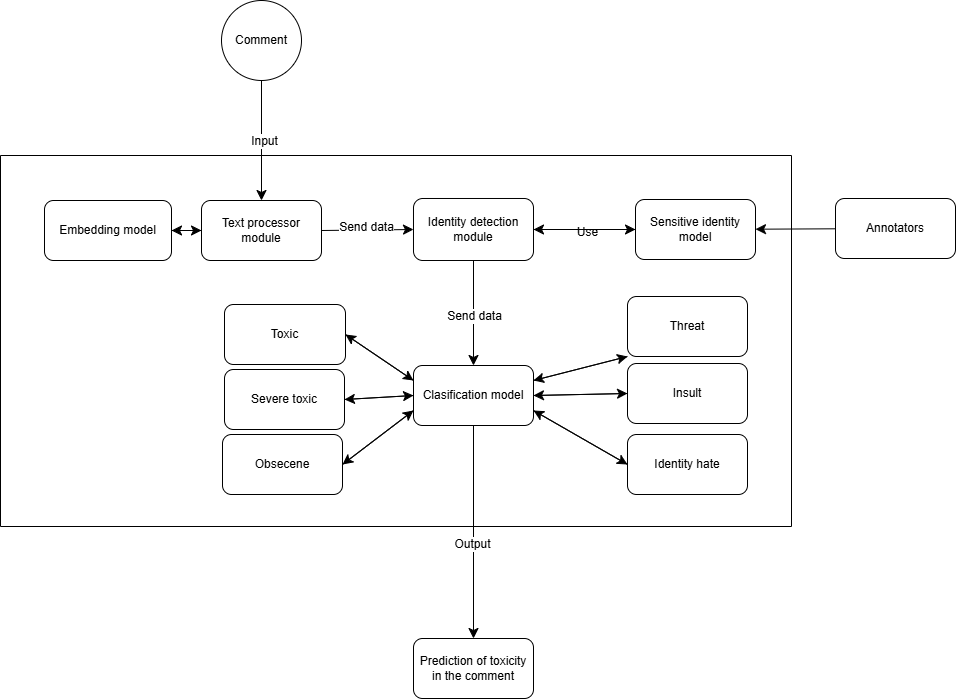
\includegraphics[width=15cm]{img/mapeoRelaciones2.drawio.png}\\[0.5cm]
\section*{3. Systems Engineering Perspective – Systemic Analysis}

This section aims to study the "Jigsaw Unintended Bias in Toxicity Classification" competition as a complex system that can be analyzed using the principles of systems engineering. This involves breaking down its components, understanding how they interact, their limits, objectives, inputs and outputs, as well as the social, technical, and ethical context of their environment, life cycle, and other aspects that have been addressed in classes throughout the semester.

\subsection*{3.1 System Definition}

From this perspective, the main system we analyze is a text classification model designed to predict the toxicity of natural language comments. However, it is not just about detecting toxicity, but also ensuring fairness: the system must minimize biases that affect certain social groups, especially those that have been historically vulnerable.

This system is composed of several elements that collaborate to fulfill a primary function: helping to moderate online content, reducing the harm caused by toxic speech while ensuring that it does not unduly punish those belonging to minorities or mentioning sensitive identities.

\subsection*{3.2 System Requirements}

\subsubsection*{Functional Requirements (What the system should do):}
\begin{itemize}
    \item Detect toxicity: Predict the toxicity of a comment (value between 0 and 1).
    \item Recognize identities: Determine whether the text mentions terms associated with gender, race, religion, or other social groups.
    \item Handle multiple annotations: Integrate opinions from multiple human annotators to estimate the collective perception of toxicity.
    \item Evaluate fairness: It should not only perform well in general, but also with comments related to minorities, avoiding systematic bias.
    \item Offer comprehensive metrics: Include overall AUC, Subgroup AUC, BPSN AUC, and BNSP AUC to evaluate performance from various angles.
\end{itemize}

\subsubsection*{Non-Functional Requirements (How it should work):}
\begin{itemize}
    \item Computational efficiency: The system must be able to handle thousands of comments in a reasonable amount of time.
    \item Scalability: It must be able to adapt to larger volumes without the need to redesign the architecture.
    \item Transparency: Its decisions must be understandable to human users and auditors.
    \item Reproducibility: The results must be exactly replicable under Kaggle's conditions.
    \item Resource constraints: It must comply with the time and memory limits imposed by the competition platform.
\end{itemize}

\subsection*{3.3 System Components}

We can divide the system into three main blocks:

\subsubsection*{Input:}
\begin{itemize}
    \item Free-text comments (\texttt{comment\_text} field).
    \item Binary columns that identify mentions of identities (male, female, Christian, black, etc.).
    \item Annotations from multiple people indicating their perception of toxicity (\texttt{toxicity\_annotator\_count}, \texttt{target}, etc.).
\end{itemize}

\subsubsection*{Processing:}
\begin{itemize}
    \item Preprocessing: Text cleaning, special character removal, tokenization, lemmatization, etc.
    \item Feature extraction: Text representation using embeddings, TF-IDF, bag-of-words, or more advanced models such as BERT.
    \item Modeling: Application of classification models (from logistic regression to deep neural networks).
    \item Metric calculation: Evaluation of model performance from a general and subgroup perspective.
\end{itemize}

\subsubsection*{Output:}
\begin{itemize}
    \item Continuous predictions between 0 and 1 indicating the probability that a comment is toxic.
    \item Analytical reports by subgroup, visualizations, and bias metrics.
\end{itemize}

\subsection*{3.4 System Environment}

\subsubsection*{Target users:}
Social platform moderators, AI ethics researchers, developers of automatic moderation systems.

\subsubsection*{External factors:}
\begin{itemize}
    \item Linguistic changes (new forms of insult, idioms).
    \item Cultural differences (what is offensive in one region may not be offensive in another).
    \item Legislative changes regarding freedom of expression or content moderation.
    \item Data sensitivity: Comments contain explicit references to identity, religion, or race, so ethical handling is crucial.
\end{itemize}

\subsection*{3.5 System Restrictions}

\subsubsection*{Technical:}
\begin{itemize}
    \item Limited resources when running the code (memory and time) on Kaggle kernels.
    \item The use of any additional data not provided by the organizers is prohibited.
\end{itemize}

\subsubsection*{Evaluative:}
\begin{itemize}
    \item The metrics used by the competition prioritize not only accuracy but also the fairness of the model across different subgroups.
\end{itemize}

\subsubsection*{Human:}
\begin{itemize}
    \item Labels come from humans with different backgrounds and criteria. The perception of toxicity is not universal.
\end{itemize}

\subsection*{3.6 System Lifecycle}

\subsubsection*{Phase: What this competition entails}
\begin{itemize}
    \item \textbf{Design:} Objectives are set (detecting toxicity and reducing bias). Inputs, outputs, and constraints are defined.
    \item \textbf{Development:} The complete pipeline is built: data cleaning, model selection, and metrics definition.
    \item \textbf{Validation:} Models are tested with different configurations, measuring overall performance and performance by subgroup.
    \item \textbf{Implementation:} (Although not a direct part of the challenge, in a real-life scenario, it would be integrated into an automated moderation system.)
    \item \textbf{Maintenance:} (Hypothetical) The model would be updated with new data, reviewed for biases, and adapted to cultural changes.
\end{itemize}

\subsection*{3.7 Ethical and Social Considerations}

These types of systems do not operate in a vacuum: they analyze human language, which is loaded with culture, emotions, and subjectivity. Therefore, ethical analysis is key.

\begin{itemize}
    \item \textbf{Risk of algorithmic bias:} A poorly trained model may penalize certain groups more heavily, even if their language is not more toxic.
    \item \textbf{False positives:} A legitimate comment can be removed simply for mentioning an identity.
    \item \textbf{False negatives:} Subtle offensive comments (such as sarcasm or double entendres) may go unnoticed.
    \item \textbf{Negative feedback:} If the system reinforces historical biases, it may amplify harm rather than mitigate it.
\end{itemize}

In short, the system must try to understand not only what is being said, but also how and who is saying it, always with a responsible and empathetic approach.

\section*{4. Sensitivity Analysis}

This analysis is extremely important when training machine learning models because it helps us understand how much each decision we make (for example, how we prepare the text, what parameters we use, etc.) affects the model's final result. In the case of this Jigsaw competition, where we seek to detect toxic comments without indulging in bias, this is key.

\subsection*{4.1. What affects the model}

There are several decisions that can make our model perform better or worse. Here are some of the main ones:

\subsubsection*{Text representation:}
The way we convert the text into something the computer can understand is critical. Some common techniques we tested were:
\begin{itemize}
    \item TF-IDF: basically gives more weight to words that appear frequently in a comment but are not as common in all texts.
    \item Word Embeddings (such as Word2Vec or GloVe): convert words into vectors that "understand" the meaning of words based on how they are used.
    \item BERT: This is more advanced because it takes into account the context of each word within the sentence.
\end{itemize}
Depending on the technique you use, the model will understand things like sarcasm or double entendres better or worse.

\subsubsection*{Model hyperparameters:}
These are like the "controls" we use to fine-tune how the model learns. Some examples:
\begin{itemize}
    \item Learning rate: how quickly the model adapts to errors.
    \item Batch size: how many comments the model sees before updating.
    \item Epochs: how many times it goes through the entire dataset.
    \item Regularization: so that the model doesn't retain the exact memory of the data and can generalize.
\end{itemize}
If you don't choose these correctly, your model may fail due to over- or under-learning.

\subsubsection*{Text preprocessing:}
Before training, the text must be neat. Some things we did were:
\begin{itemize}
    \item Tokenization: splitting the comment into words or phrases.
    \item Lemmatization or stemming: Reducing words to their basic form (for example, “insulting” $\rightarrow$ “insult”).
    \item Removing common words that don't contribute much (“and,” “the,” “of”).
\end{itemize}
Doing this well improves the quality of the data we use for training, and this is noticeable in the final result.

\subsubsection*{Strategies to reduce bias:}
Since the goal is to prevent the model from being unfair to certain groups, there are techniques that help:
\begin{itemize}
    \item Reweighting: Giving more weight to certain examples to maintain balance between different groups (for example, not all comments with the word “Muslim” are labeled as toxic).
    \item Threshold adjustment: Changing the number above which we consider something toxic.
    \item Adversarial debiasing: Training the model to ignore people's identities when making predictions.
\end{itemize}
Each strategy works differently depending on the model and the data, so it's worth testing.

\subsection*{4.2. How we measure all of this}

There are tools that allow us to see the impact of these parameters and decisions. Some of them are:

\subsubsection*{Cross-validation:}
We divide the dataset into parts and train using different combinations. This way, we ensure that the model doesn't rely solely on one group of data and becomes more general.

\subsubsection*{Learning curves:}
We create graphs to see how the model performs as it sees more data. This helps us understand if we are overtraining (overfitting) or if the model lacks the ability to learn (underfitting).

\subsubsection*{Feature importance:}
This allows us to see which words or groups of words (n-grams) are most useful for the model to detect toxicity. This can also give us clues about bias (for example, if the word "gay" appears as very important for detecting toxicity... something is wrong).

\subsubsection*{Fairness metrics:}
These help us see if the model treats all groups equally. Some metrics we use:
\begin{itemize}
    \item Equal opportunity: that the true hit rate is equal between groups.
    \item Demographic parity: that positive predictions are distributed equally.
    \item Disparate impact: compares how much a disadvantaged group is affected compared to a privileged one.
\end{itemize}
With this, we can compare how fair a model is and whether our strategies to reduce bias are working.

\subsubsection*{Local sensitivity analysis:}
Here, what we do is change a comment slightly (for example, change a word) and see if the model completely changes the prediction. If that happens, it's because the model isn't very stable or is too sensitive to specific words.

\section*{5. Chaos and complexity theory}

This part sounds a bit more theoretical, but it makes sense when applied to how a machine learning model works.
In essence, chaos theory says that in complex, nonlinear systems (like human language), a small change can have a huge effect. And ML models, especially in NLP tasks, are full of these situations.

\subsection*{5.1. Chaotic or Unpredictable Elements}

\subsubsection*{Language Variability:}
The way we speak is a mess (and a beautiful one at that). It can contain irony, sarcasm, puns, insults disguised as jokes, etc. The model often can't capture these subtleties. Furthermore, the dataset includes strong comments, and that adds a lot of "noise."

\subsubsection*{Subjectivity of Toxicity:}
What may be offensive to one person may not be to another. In the dataset, toxicity is based on how many annotators marked a comment as toxic. This means that even from the labeling, there is some ambiguity.

\subsubsection*{Data Biases:}
Training data may contain biases that reflect real prejudices. For example, if more comments with certain identities were labeled as toxic in the original data, the model may learn that as if it were correct and continue reproducing those biases.

\subsubsection*{Interaction between participants:}
As this is a public competition, each person or team tries new things, and this means the environment is constantly changing. Ideas are shared, and this can cause the "state of the art" to change from one week to the next. It's a dynamic system.

\subsection*{5.2. Random or feedback processes}

\subsubsection*{Text generation:}
The way toxic comments are generated is not predictable. It depends on the mood of the person writing it, the context, etc. In other words, it's not something we can easily model.

\subsubsection*{Annotation process:}
Labeling data also has its random side. The person annotating it may be tired, distracted, or have their own biases. Even the same comment viewed by two people can receive different labels. This is why multiple annotators are sometimes used per comment.

\subsubsection*{Model Training:}
The learning process of a model is not linear. Small changes in the data, parameters, or even the order in which examples are viewed can significantly change the outcome.

\subsubsection*{Competition Dynamics:}
Because it's an open competition, one team's results and strategies can influence others. This creates a kind of feedback loop where everyone constantly improves and adapts.

\end{document}
